\documentclass{article}

\usepackage[italian]{babel}
\usepackage[letterpaper,top=2cm,bottom=2cm,left=3cm,right=3cm,marginparwidth=1.75cm]{geometry}
\usepackage{amsmath}
\usepackage{graphicx}
\usepackage{subcaption}
\usepackage{textcomp}
\usepackage{float}
\usepackage{ragged2e}
\usepackage[dvipsnames]{xcolor}
\usepackage{fancyhdr}
\usepackage[colorlinks=true, allcolors=blue,
            pdfauthor={Matteo Drago},
            pdftitle={Malga Fornasa Alta},
            pdfsubject={Diario bivacchi e trekking},
            pdfkeywords={bivacco, montagna, trekking, diario}]{hyperref}
                
\title{\textbf{Malga Fornasa Alta - 1892 m s.l.m}}
\author{Matteo Drago}

% ==========================================================
% Impostazioni per il logo in ogni pagina
% ==========================================================
\pagestyle{fancy}
\fancyhf{} % Pulisce tutti i campi di intestazione e piè di pagina
\fancyhead[R]{
\includegraphics[height=1.5cm]{images/toothless.jpeg}} % Posiziona il logo a destra (R) nell'intestazione
\renewcommand{\headrulewidth}{0pt} % Rimuove la linea orizzontale nell'intestazione (opzionale)


\begin{document}
\maketitle
\thispagestyle{fancy} % Aggiungi questa riga

\begin{abstract}
Questo documento raccoglie e organizza le informazioni che ho acquisito nel corso degli anni sui bivacchi, basate sulle mie esperienze dirette. Sebbene non si proponga come una guida esaustiva e perfetta, offre il minimo indispensabile per una buona vita in bivacco, con consigli pratici e diretti per chiunque desideri affrontare al meglio queste pazze ma piacevoli avventure.
\end{abstract}

\section{Il bivacco}

% ==========================================================
% Immagine a sinistra, testo a destra allineato in alto
% ==========================================================
\noindent
\begin{minipage}[t]{0.45\textwidth}
  \vspace{0pt} % forza l'allineamento in alto
  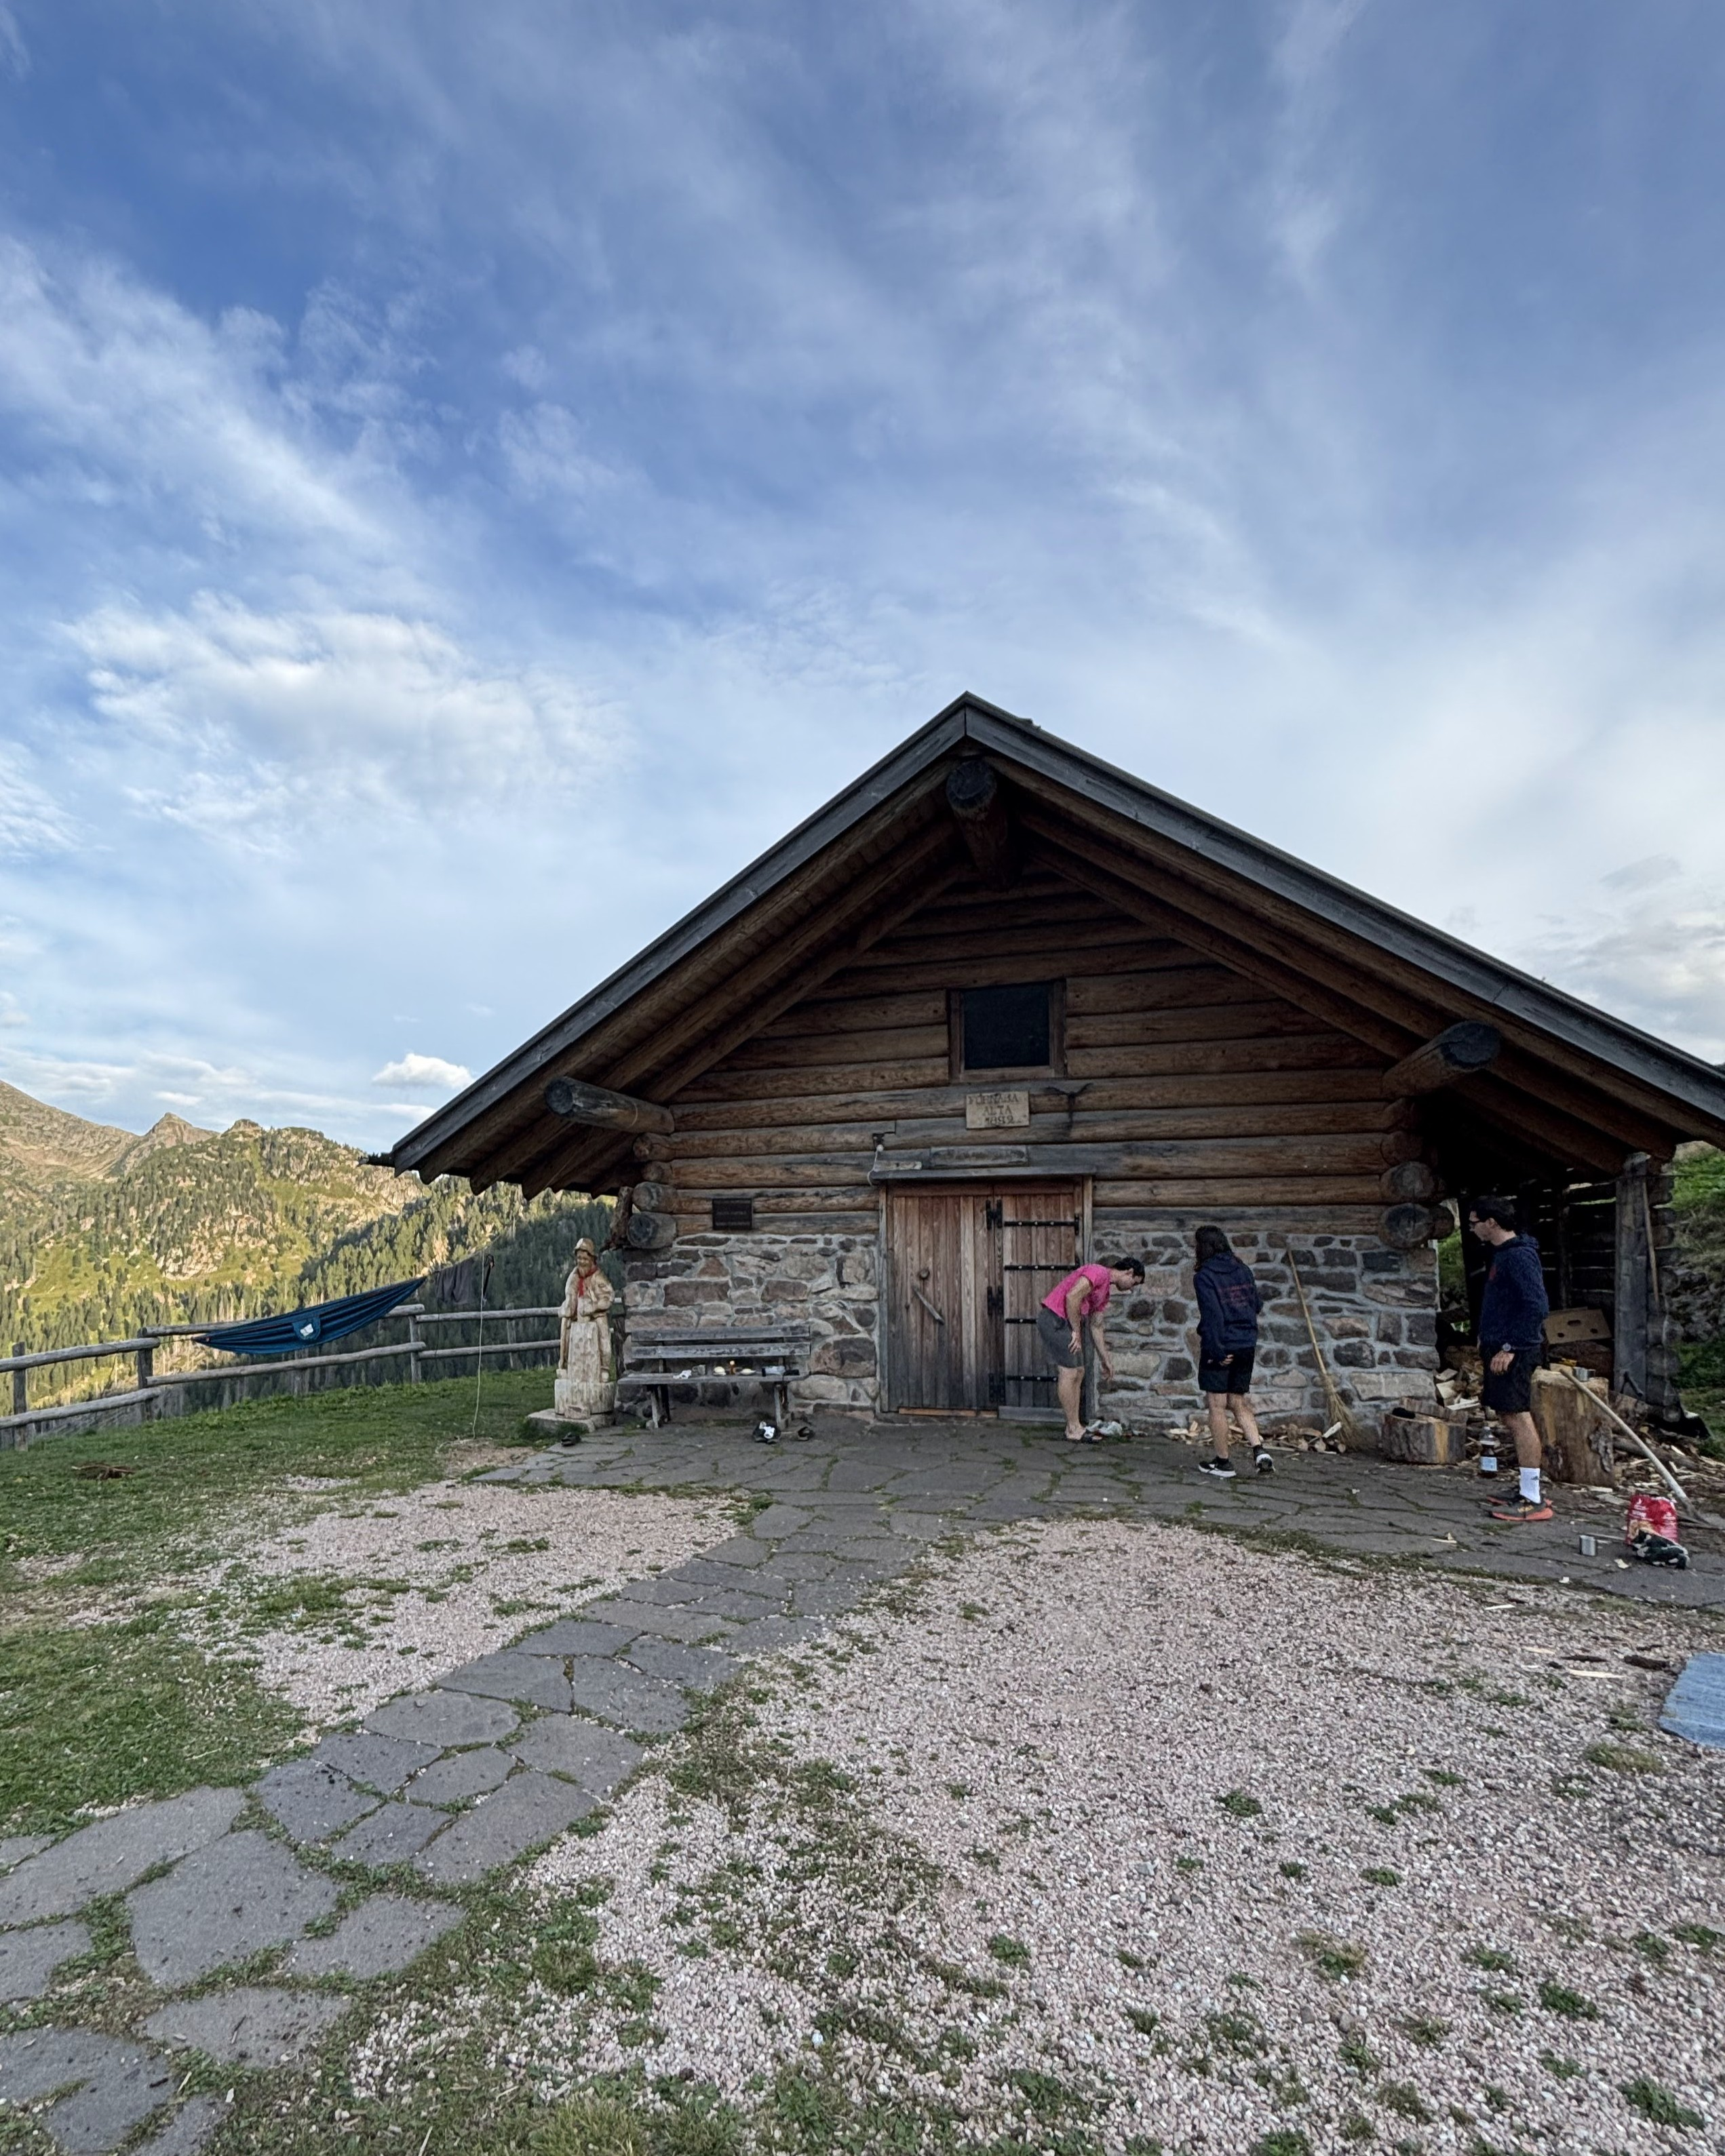
\includegraphics[width=\linewidth]{images/bivacco.jpg}
\end{minipage}%
\hfill
\begin{minipage}[t]{0.5\textwidth}
  \vspace{0pt} % forza l'allineamento in alto
  
  Gruppo montuoso\\
  \textbf{\large Catena dei Lagorai}
  \\[1em] % Aggiunge una riga vuota qui
  Località\\
  \textbf{\large Val di Cadino}
  \\[1em] % Aggiunge una riga vuota qui
  Comune catastale\\  
  \textbf{\large Valfloriana}
  \\[1em] % Aggiunge una riga vuota qui
  Comune proprietario\\  
  \textbf{\large Fornace}
  \\[1em] % Aggiunge una riga vuota qui
  Altezza\\  
  \textbf{\large 1892 m s.l.m.}
  \\[1em] % Aggiunge una riga vuota qui
  Apertura\\  
  \textbf{\large Non gestito, sempre aperto}

\end{minipage}

\subsection{Caratteristiche}
La malga Fornasa Alta è un rifugio alpino con caratteristiche di bivacco attrezzato e assieme alla malga Valletta alta, la cugina praticamente, rappresentano quello che molti definiscono un gioiello di struttura.

Il bivacco è suddiviso in 2 piani:
\begin{itemize}
    \item \textbf{Piano terra}: ampia stanza con diversi tavoli con panche, una dispensa molto ampia e ben fornita, una cucina a gas e una stufa.
    \item \textbf{Piano superiore}: molto ampio con diverse brande in grado di ospitare comodamente circa 8-10 persone. 
    \item \textbf{Spazio esterno}: con fonte d'acqua attiva sia in estate che in inverno, una legnaia fornita, un camino e sul retro del bivacco è presente anche un "bagno-latrina".
\end{itemize}

La stufa presente è in grado di riscaldare molto facilmente tutto il bivacco e ricavare la legna non è complesso grazie alla presenza del bosco. 


\section{Come ci siamo arrivati}
\subsection{Giro 1: giro di 3 giorni tra Valletta alta e Fornasa alta}
Il bivacco è stato inserito in un giro di tre giorni che comprendeva la malga Valletta Alta e la malga Fornasa Alta.

Abbiamo parcheggiato l’auto sulla strada Provinciale 31 del Manghen, (non ho un punto specifico data la presenza di molta neve sulla strada, siamo saliti fino a quando ci era permesso, comunque potete vedere la traccia gpx) e da lì ci siamo incamminati fino a raggiungere la malga Valletta Alta. Il giorno successivo siamo ripartiti in direzione della malga Fornasa Alta per poi terminare il giro il terzo giorno, tornando al parcheggio.
Lascio le informazioni del giro completo dei 3 giorni.

\begin{figure}[htbp!]
    \centering
    % Colonna di sinistra, allineata in alto
    \begin{subfigure}[t]{0.45\textwidth}
        \centering
        \vspace{0pt} % Forziamo l'allineamento in alto
        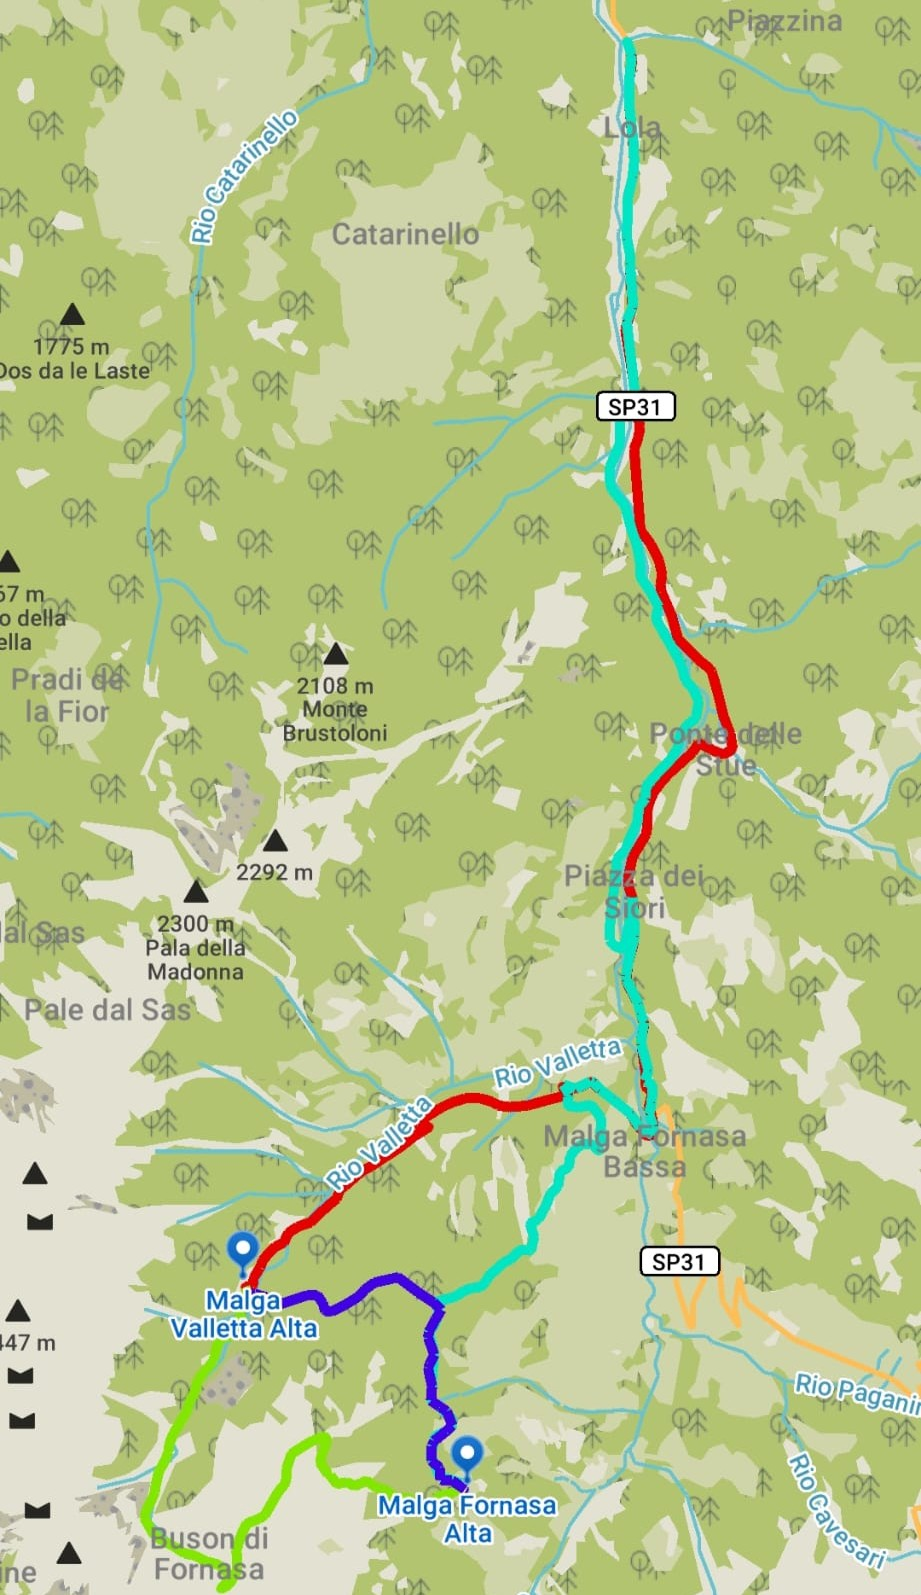
\includegraphics[width=\textwidth]{images/sentiero_mapsMe_Giro1.jpg}
        \caption{Sentiero su Maps.Me.}
        \label{fig:foto_lunga}
    \end{subfigure}
    \hfill
    % Colonna di destra, allineata in alto
    \begin{subfigure}[t]{0.45\textwidth}
        \centering
        \vspace{0pt} % Forziamo l'allineamento in alto anche qui
        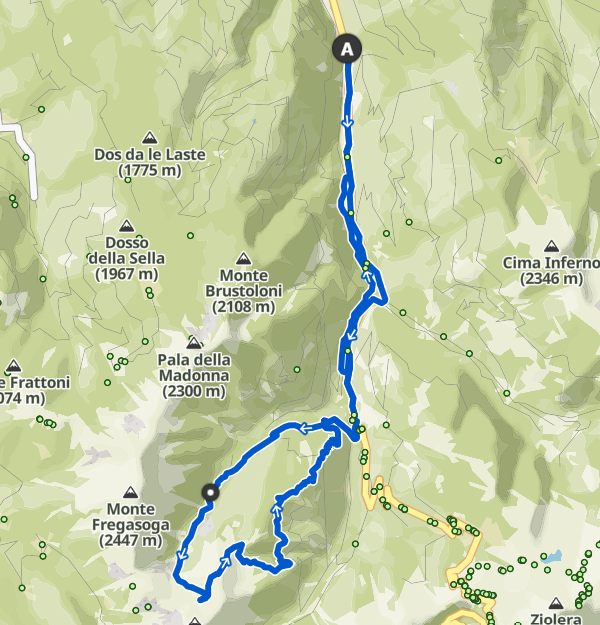
\includegraphics[width=\textwidth]{images/sentiero_komoot_Giro1.png}
        \caption{Sentiero su Komoot.}
        \label{fig:foto_corta1}
        \vspace{1em} % Aggiunge un po' di spazio tra le due foto
        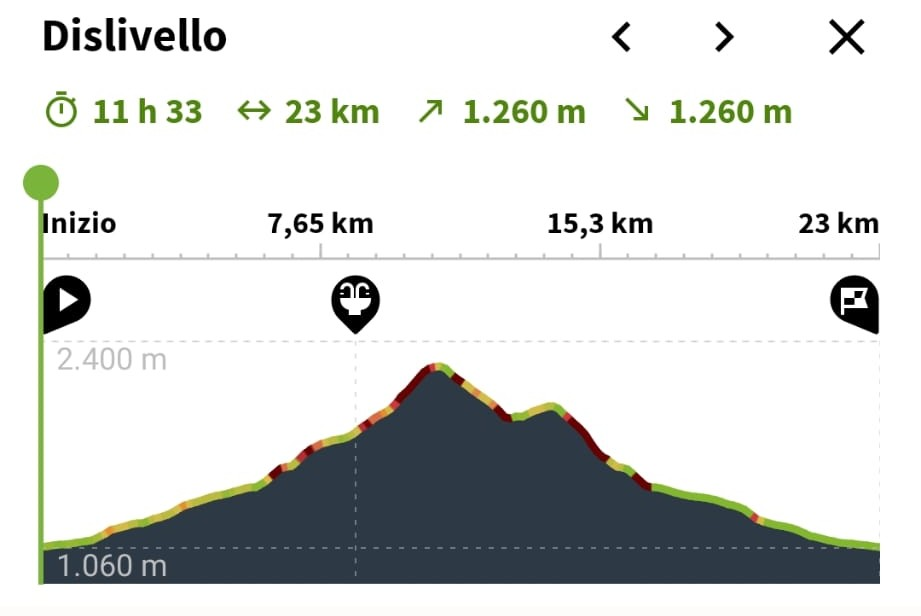
\includegraphics[width=\textwidth]{images/profilo_altimetrico_Giro1.jpg}
        \caption{Profilo altimetrico del percorso.}
        \label{fig:foto_corta2}
    \end{subfigure}
    % Didascalia generale per l'intera figura
    \caption{Il sentiero e i dettagli del percorso.}
    \label{fig:panoramica_dettagli_giro1}
\end{figure}

\subsubsection{Esperienza Personale}
La complessità di questo giro si è rivelata \textbf{molto elevata}.
Siamo partiti con poche ciaspole rispetto a quelle disponibili, convinti che la neve non fosse molta e che, in ogni caso, fosse piuttosto compatta. Mai scelta fu più sbagliata: lungo il tratto stradale la neve era effettivamente dura e battuta, ma appena ci siamo addentrati nei sentieri è diventata più abbondante e soffice.
Camminare con le ciaspole non è stato semplice, e persino restare in equilibrio da fermi richiedeva uno sforzo notevole. 

Il \textbf{primo giorno} è stato comunque gestibile: l’unica vera difficoltà è stata la salita finale verso il bivacco, che per fortuna abbiamo trovato libero e accogliente, permettendoci di riposare in vista della tappa successiva verso la malga Fornasa Alta.

Il \textbf{secondo giorno} si è rivelato molto più impegnativo. La salita era ripidissima: chi non aveva le ciaspole letteralmente “nuotava nella neve”. Abbiamo raggiunto la vetta con molta fatica e poi il bivacco, ma solo verso le 16:00, partendo alle 10:00 e senza riuscire a fermarci per pranzo per mancanza di un luogo adatto alla sosta.

Il \textbf{terzo giorno} ci ha messo di fronte a un’ulteriore difficoltà. Il sentiero che avremmo dovuto seguire era completamente ostruito dagli alberi abbattuti dalla tempesta Vaia: tronchi caduti e ramaglie bloccavano ogni passaggio. Abbiamo quindi dovuto improvvisare un percorso alternativo, districandoci tra rovi, salite ripide e deviazioni forzate. È stato un cammino lento e faticoso, ma alla fine siamo riusciti a ritornare al parcheggio, stanchi ma soddisfatti di aver concluso il giro.


\subsection{Giro 2: dal rifugio del passo Manghen alla malga Fornasa alta}
Abbiamo parcheggiato la macchina di fronte al lago di Cadinei, presso il rifugio del passo Manghen, e da li siamo partiti per un giro ad anello con l'obiettivo di raggiungere la malga Fornasa alta.

\begin{figure}[htbp!]
    \centering
    % Colonna di sinistra, allineata in alto
    \begin{subfigure}[t]{0.45\textwidth}
        \centering
        \vspace{0pt} % Forziamo l'allineamento in alto
        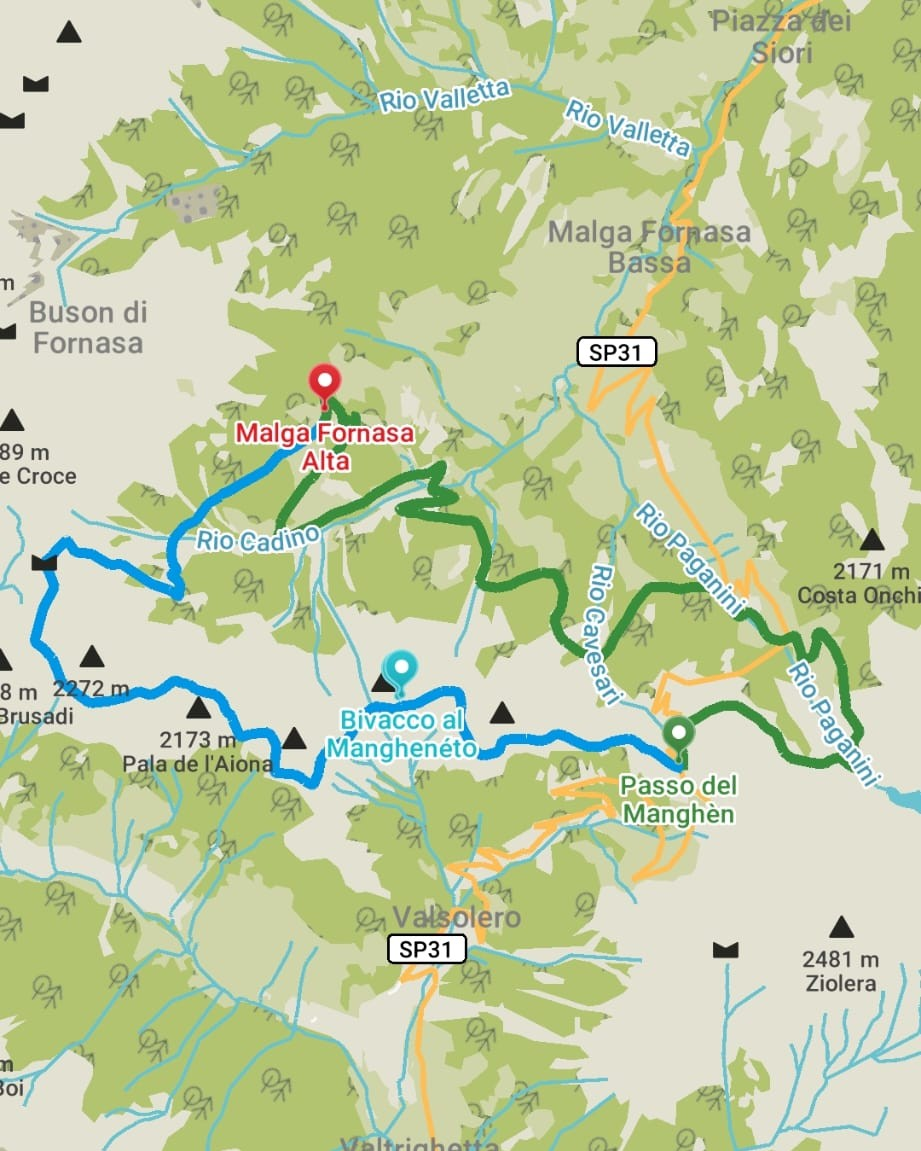
\includegraphics[width=\textwidth]{images/sentiero_mapsMe_Giro2.jpg}
        \caption{Sentiero su Maps.Me.}
        \label{fig:foto_lunga2}
    \end{subfigure}
    \hfill
    % Colonna di destra, allineata in alto
    \begin{subfigure}[t]{0.45\textwidth}
        \centering
        \vspace{0pt} % Forziamo l'allineamento in alto anche qui
        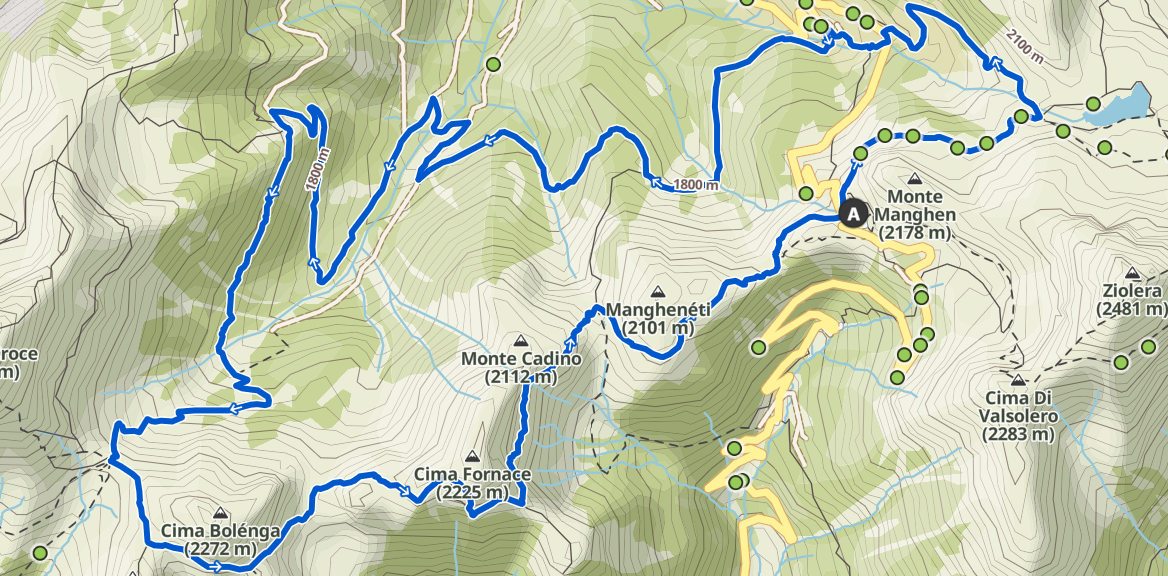
\includegraphics[width=\textwidth]{images/sentiero_komoot_Giro2.png}
        \caption{Sentiero su Komoot.}
        \label{fig:foto_corta3}
        \vspace{1em} % Aggiunge un po' di spazio tra le due foto
        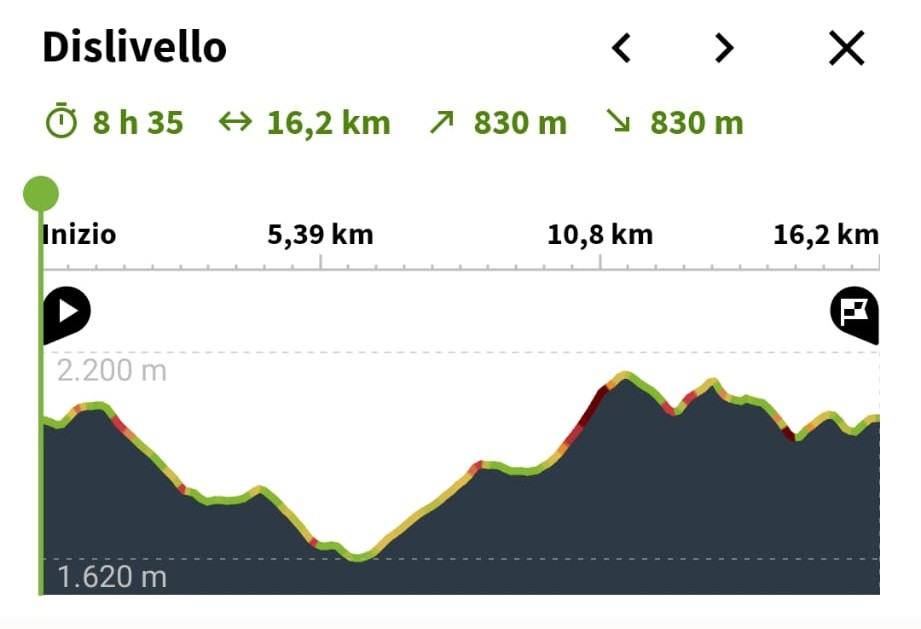
\includegraphics[width=\textwidth]{images/profilo_altimetrico_Giro2.jpg}
        \caption{Profilo altimetrico del percorso.}
        \label{fig:foto_corta4}
    \end{subfigure}
    % Didascalia generale per l'intera figura
    \caption{Il sentiero e i dettagli del percorso.}
    \label{fig:panoramica_dettagli_giro2}
\end{figure}

\subsubsection{Esperienza Personale}
Siamo partiti dal rifugio al \textbf{Passo del Manghen} subito dopo pranzo. Il cammino si è rivelato piacevole e immerso in un paesaggio estivo stupendo, molto diverso dall’atmosfera invernale della nostra precedente visita.

Siamo arrivati al bivacco verso le 16:00. Inizialmente eravamo soli, ma in serata siamo stati raggiunti da tre ragazzi accompagnati da un cane. Il bivacco, come sempre, si è confermato un vero gioiello: ampio, ben tenuto, con la comodità della luce e soprattutto dell’acqua.

Il giorno seguente siamo ripartiti in mattinata per fare ritorno alla macchina. Complice il caldo, abbiamo deciso di concludere la giornata con una sosta rinfrescante al lago di Caldonazzo.


\section{Non ti scordar di me}
\textbf{\textcolor{BurntOrange}{Ricorda: il bivacco è un bene comune. Il suo futuro dipende dal rispetto e dal senso civico dei visitatori. Usalo con cura e lascialo più pulito di come l'hai trovato.}}

\section{Alcune foto}

% Sezione Alcune foto

\begin{figure}[htbp!]
    \centering
    % Prima riga: Due foto (QUESTA È LA PRIMA FIGURA)
    \begin{subfigure}[b]{0.45\textwidth}
        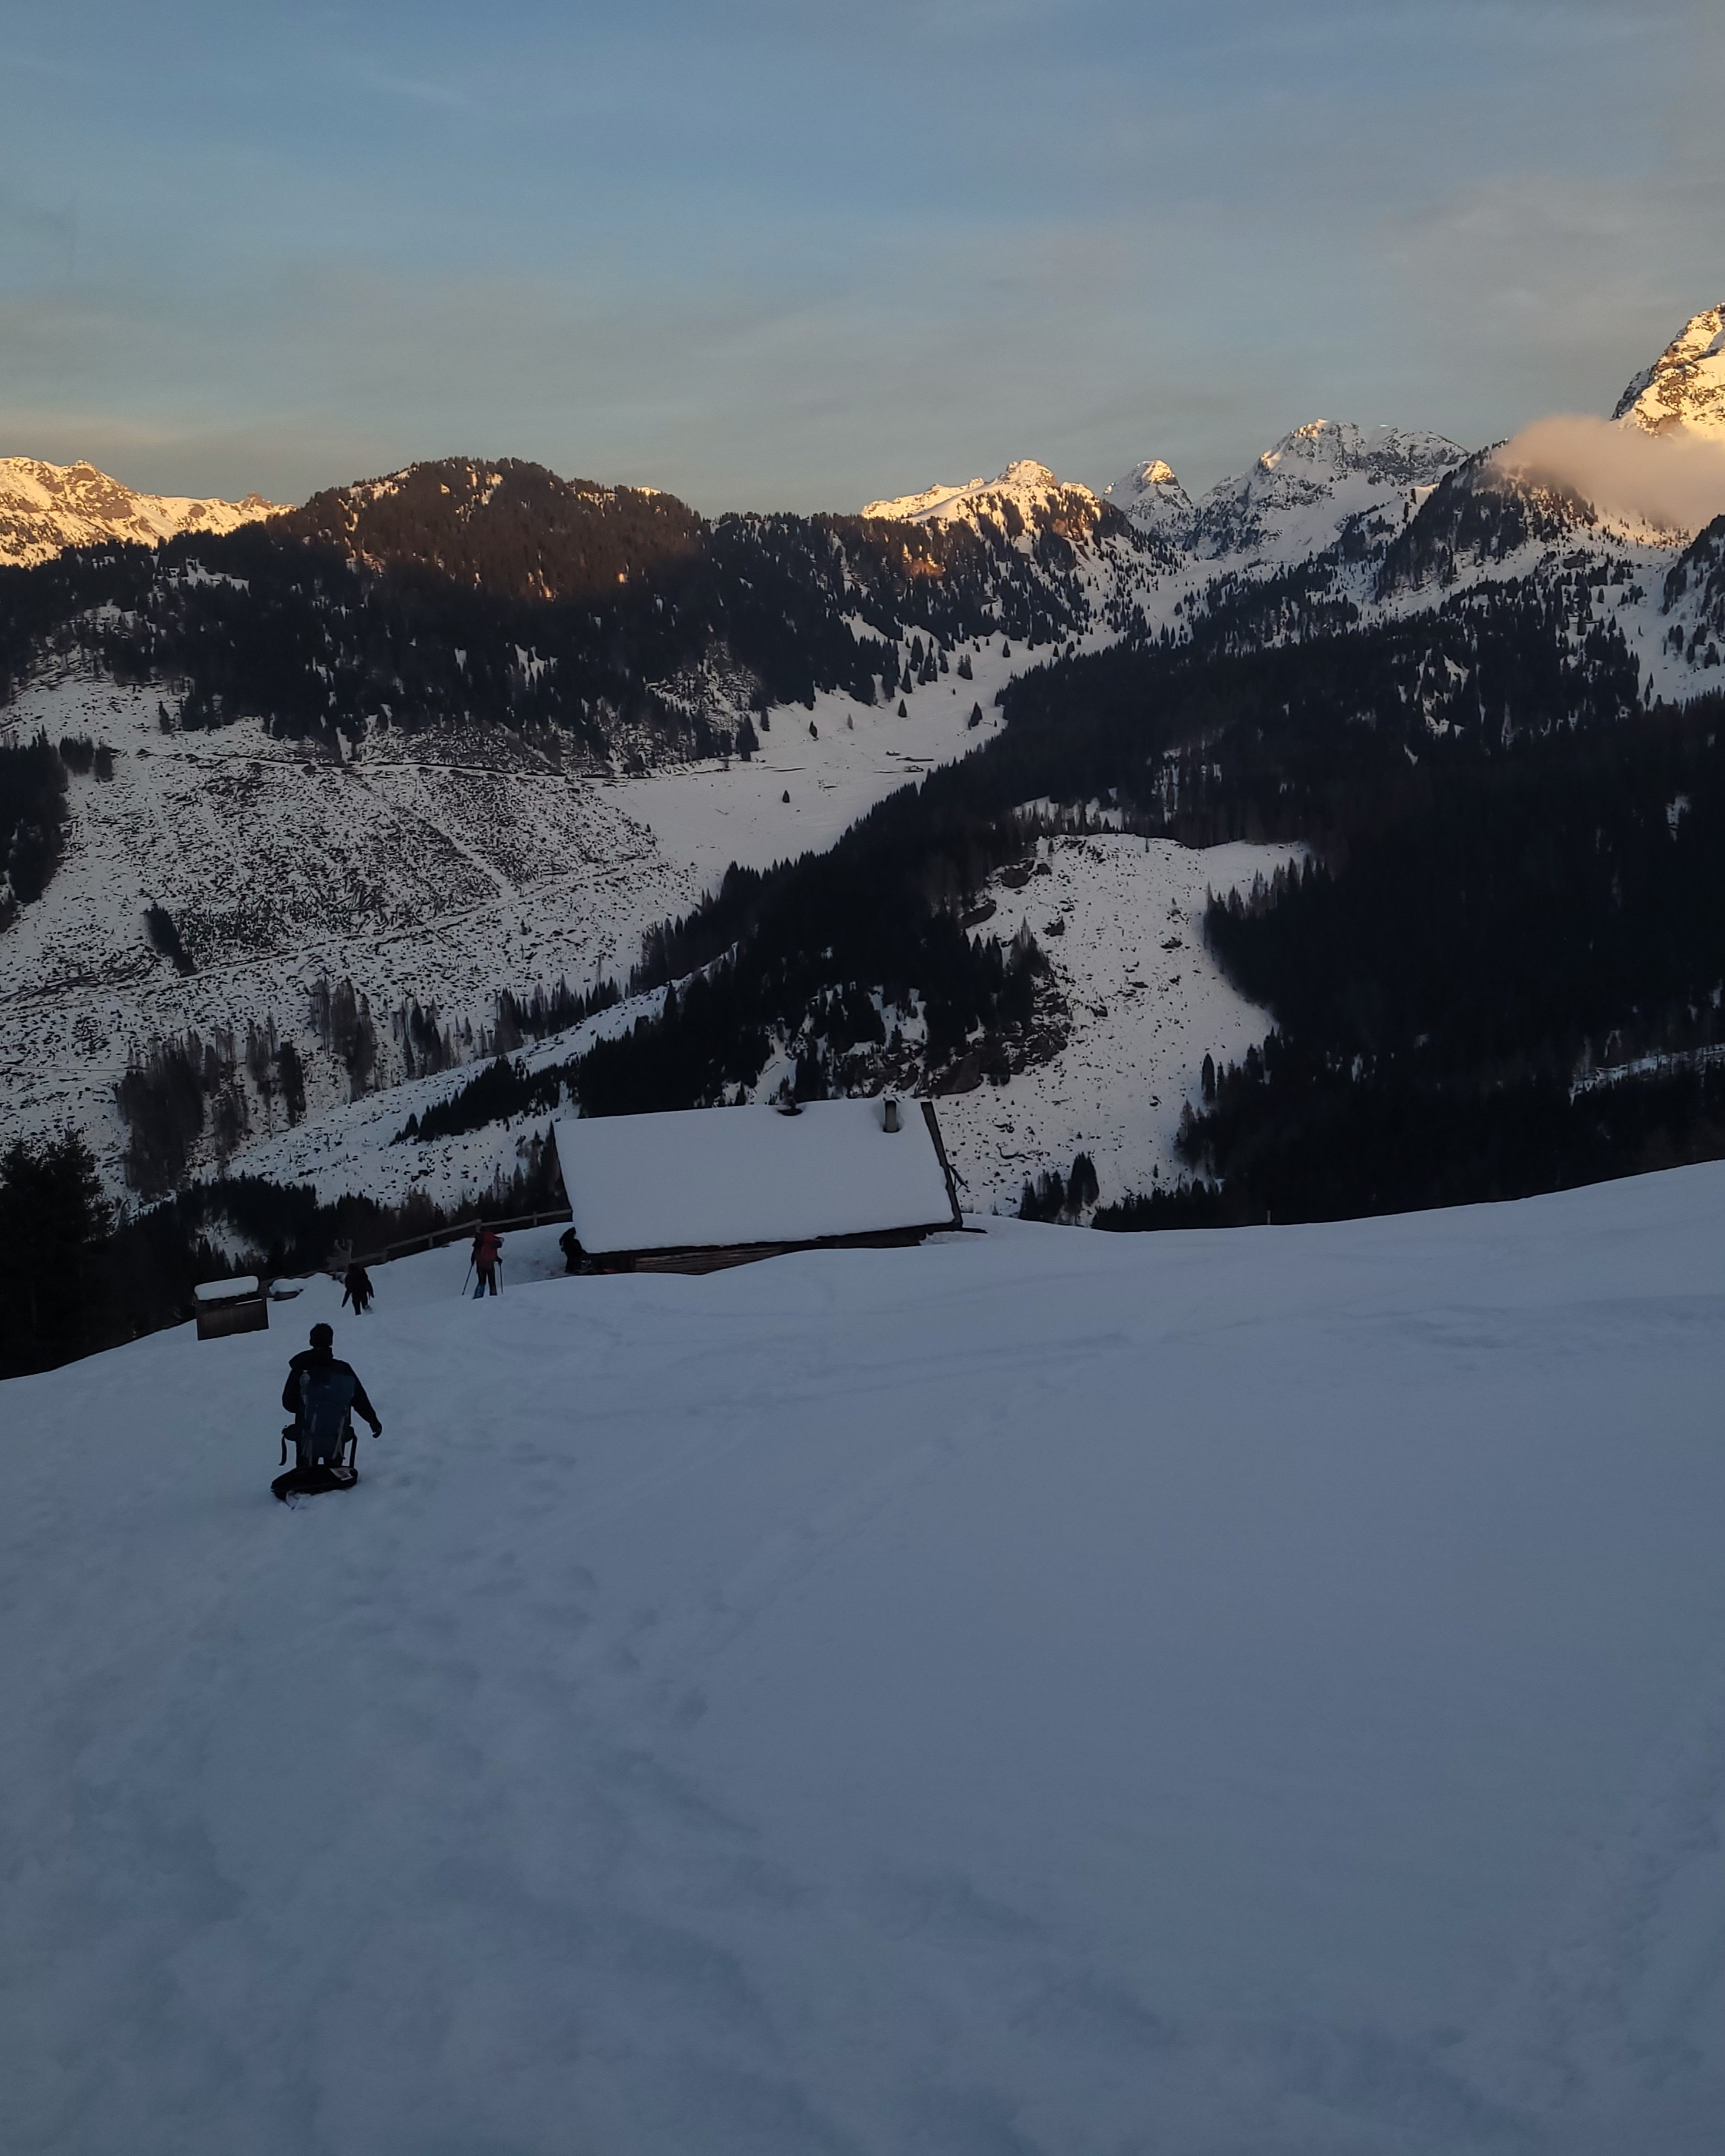
\includegraphics[width=\textwidth]{images/foto_bivacco.jpg}
        \caption{Vista del bivacco.}
    \end{subfigure}
    \hfill
    \begin{subfigure}[b]{0.45\textwidth}
        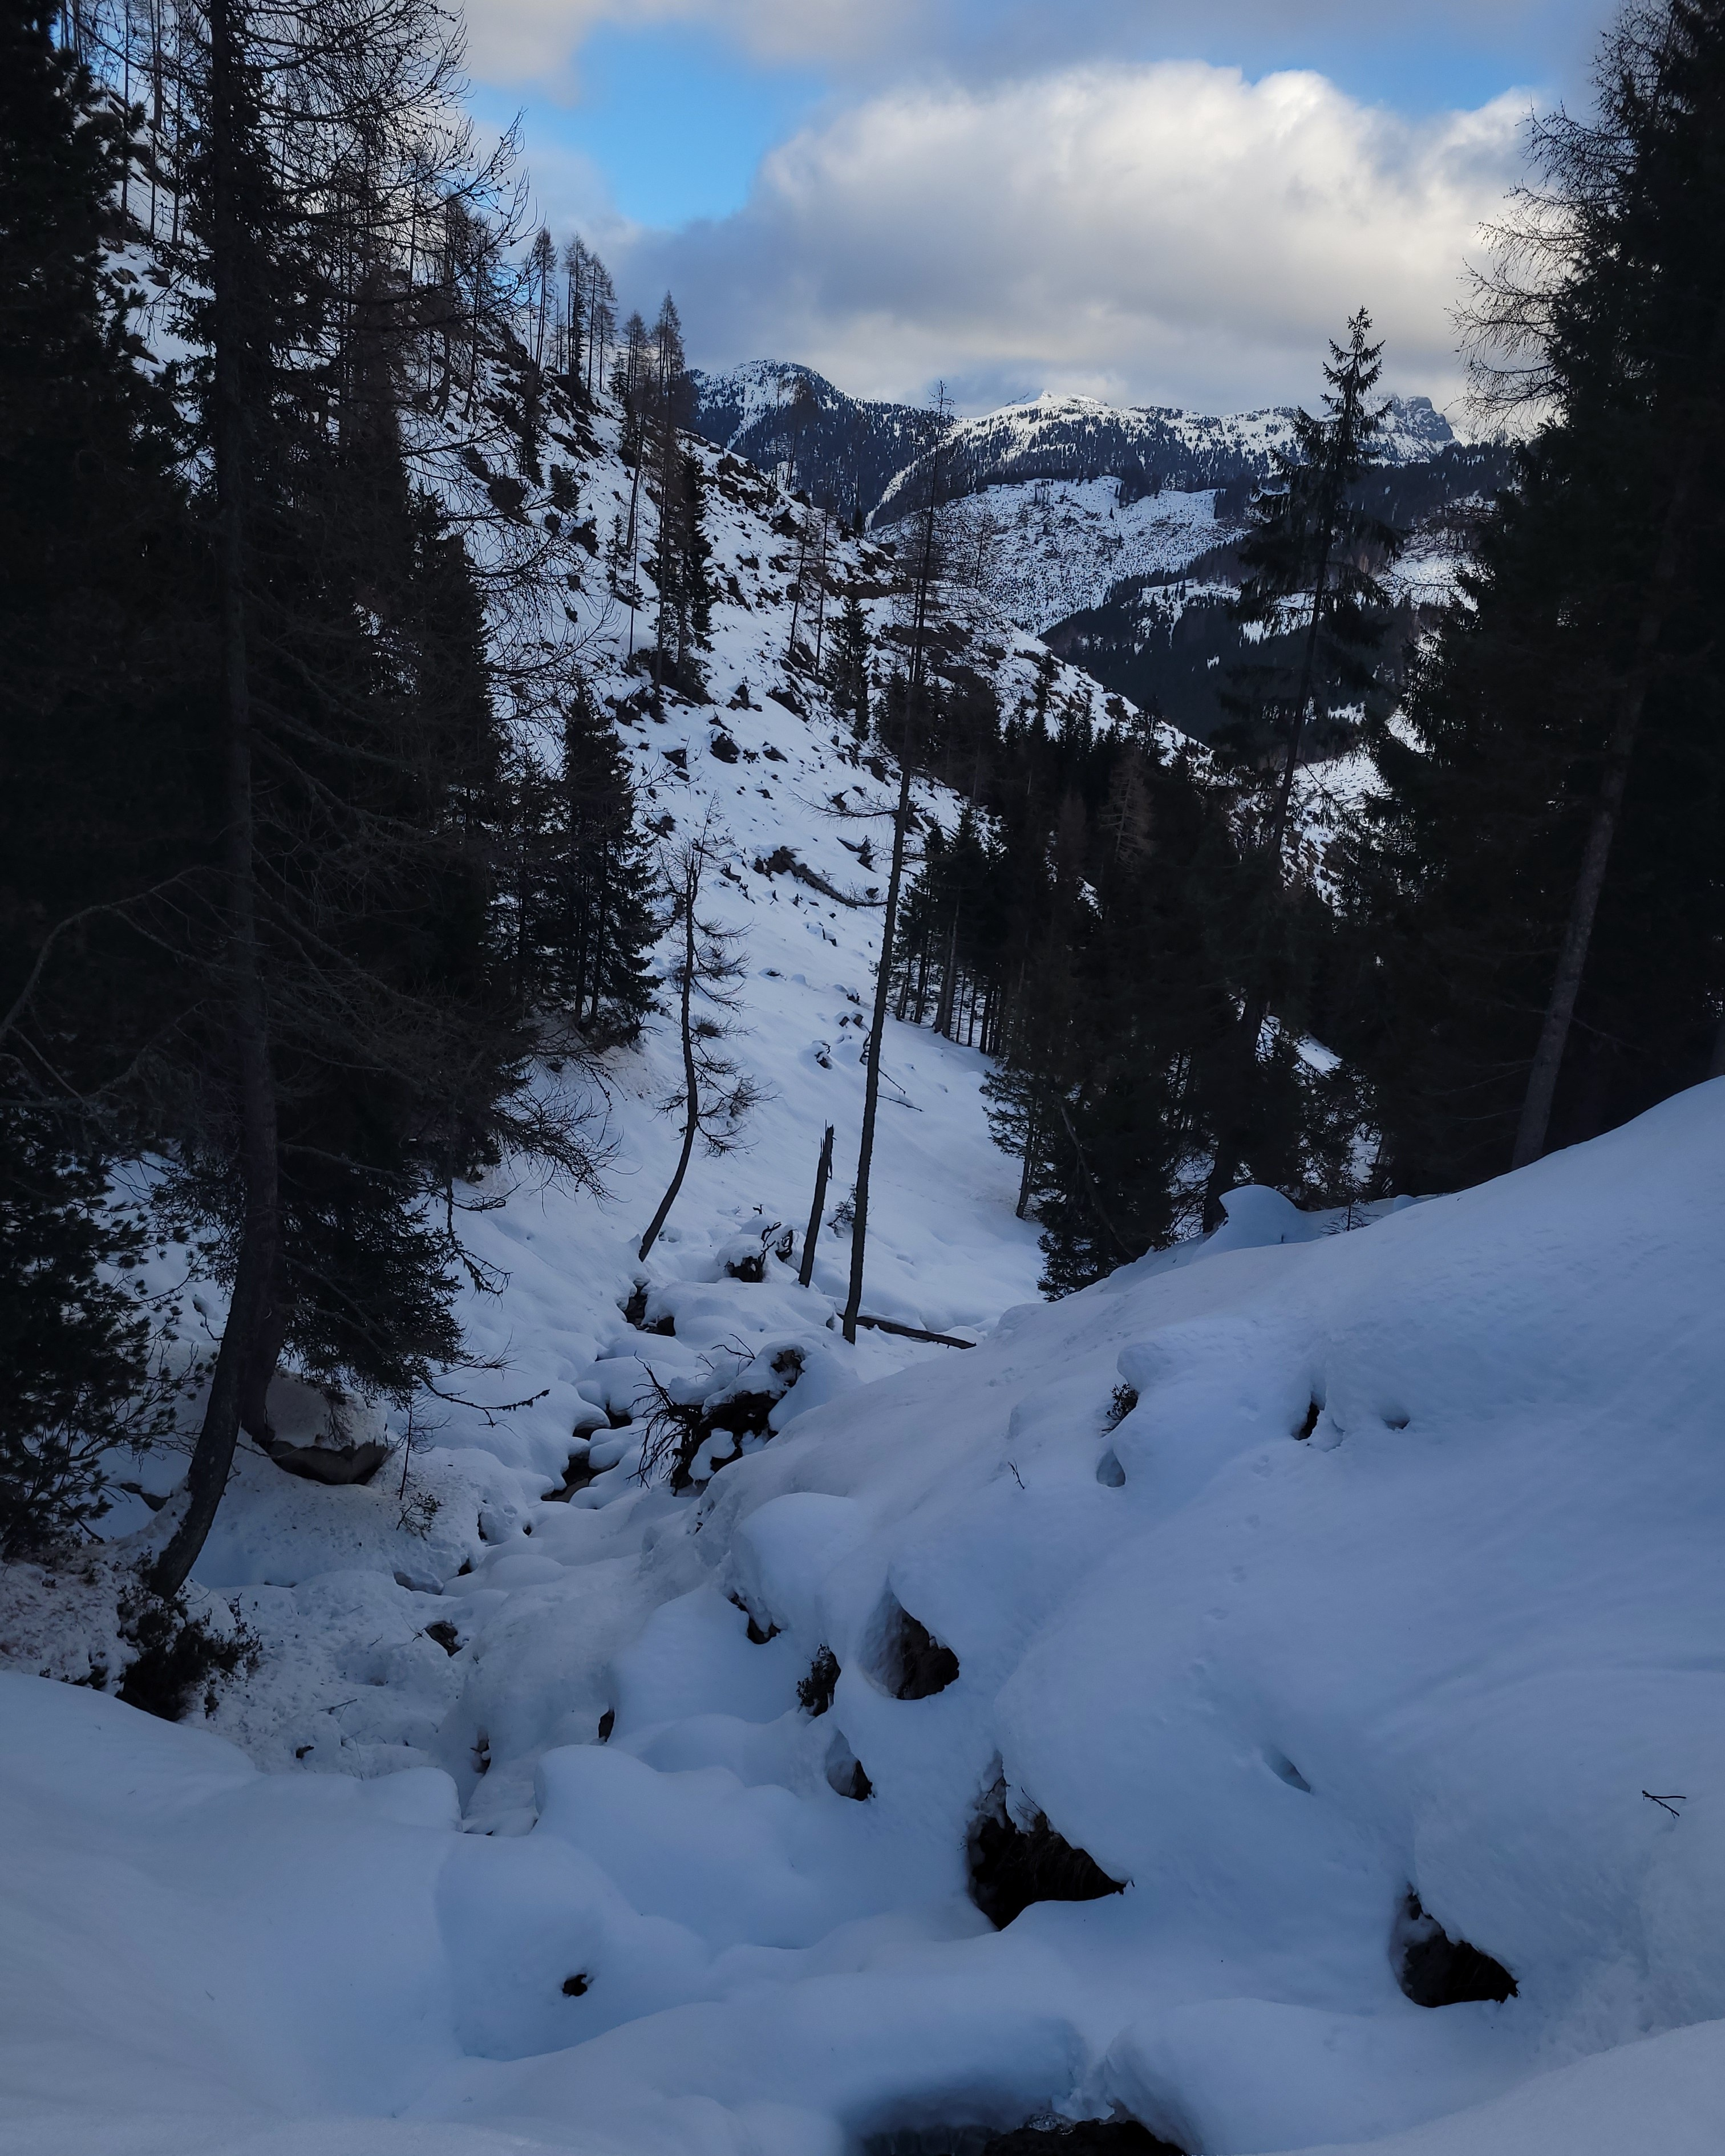
\includegraphics[width=\textwidth]{images/foto_paesaggio.jpg}
        \caption{Paesaggio.}
    \end{subfigure}

    \caption{Alcune foto.}
\end{figure}


\begin{figure}[H]
    \centering
    % Seconda riga: Tre foto (QUESTA È LA SECONDA FIGURA)
    \begin{subfigure}[b]{0.45\textwidth}
        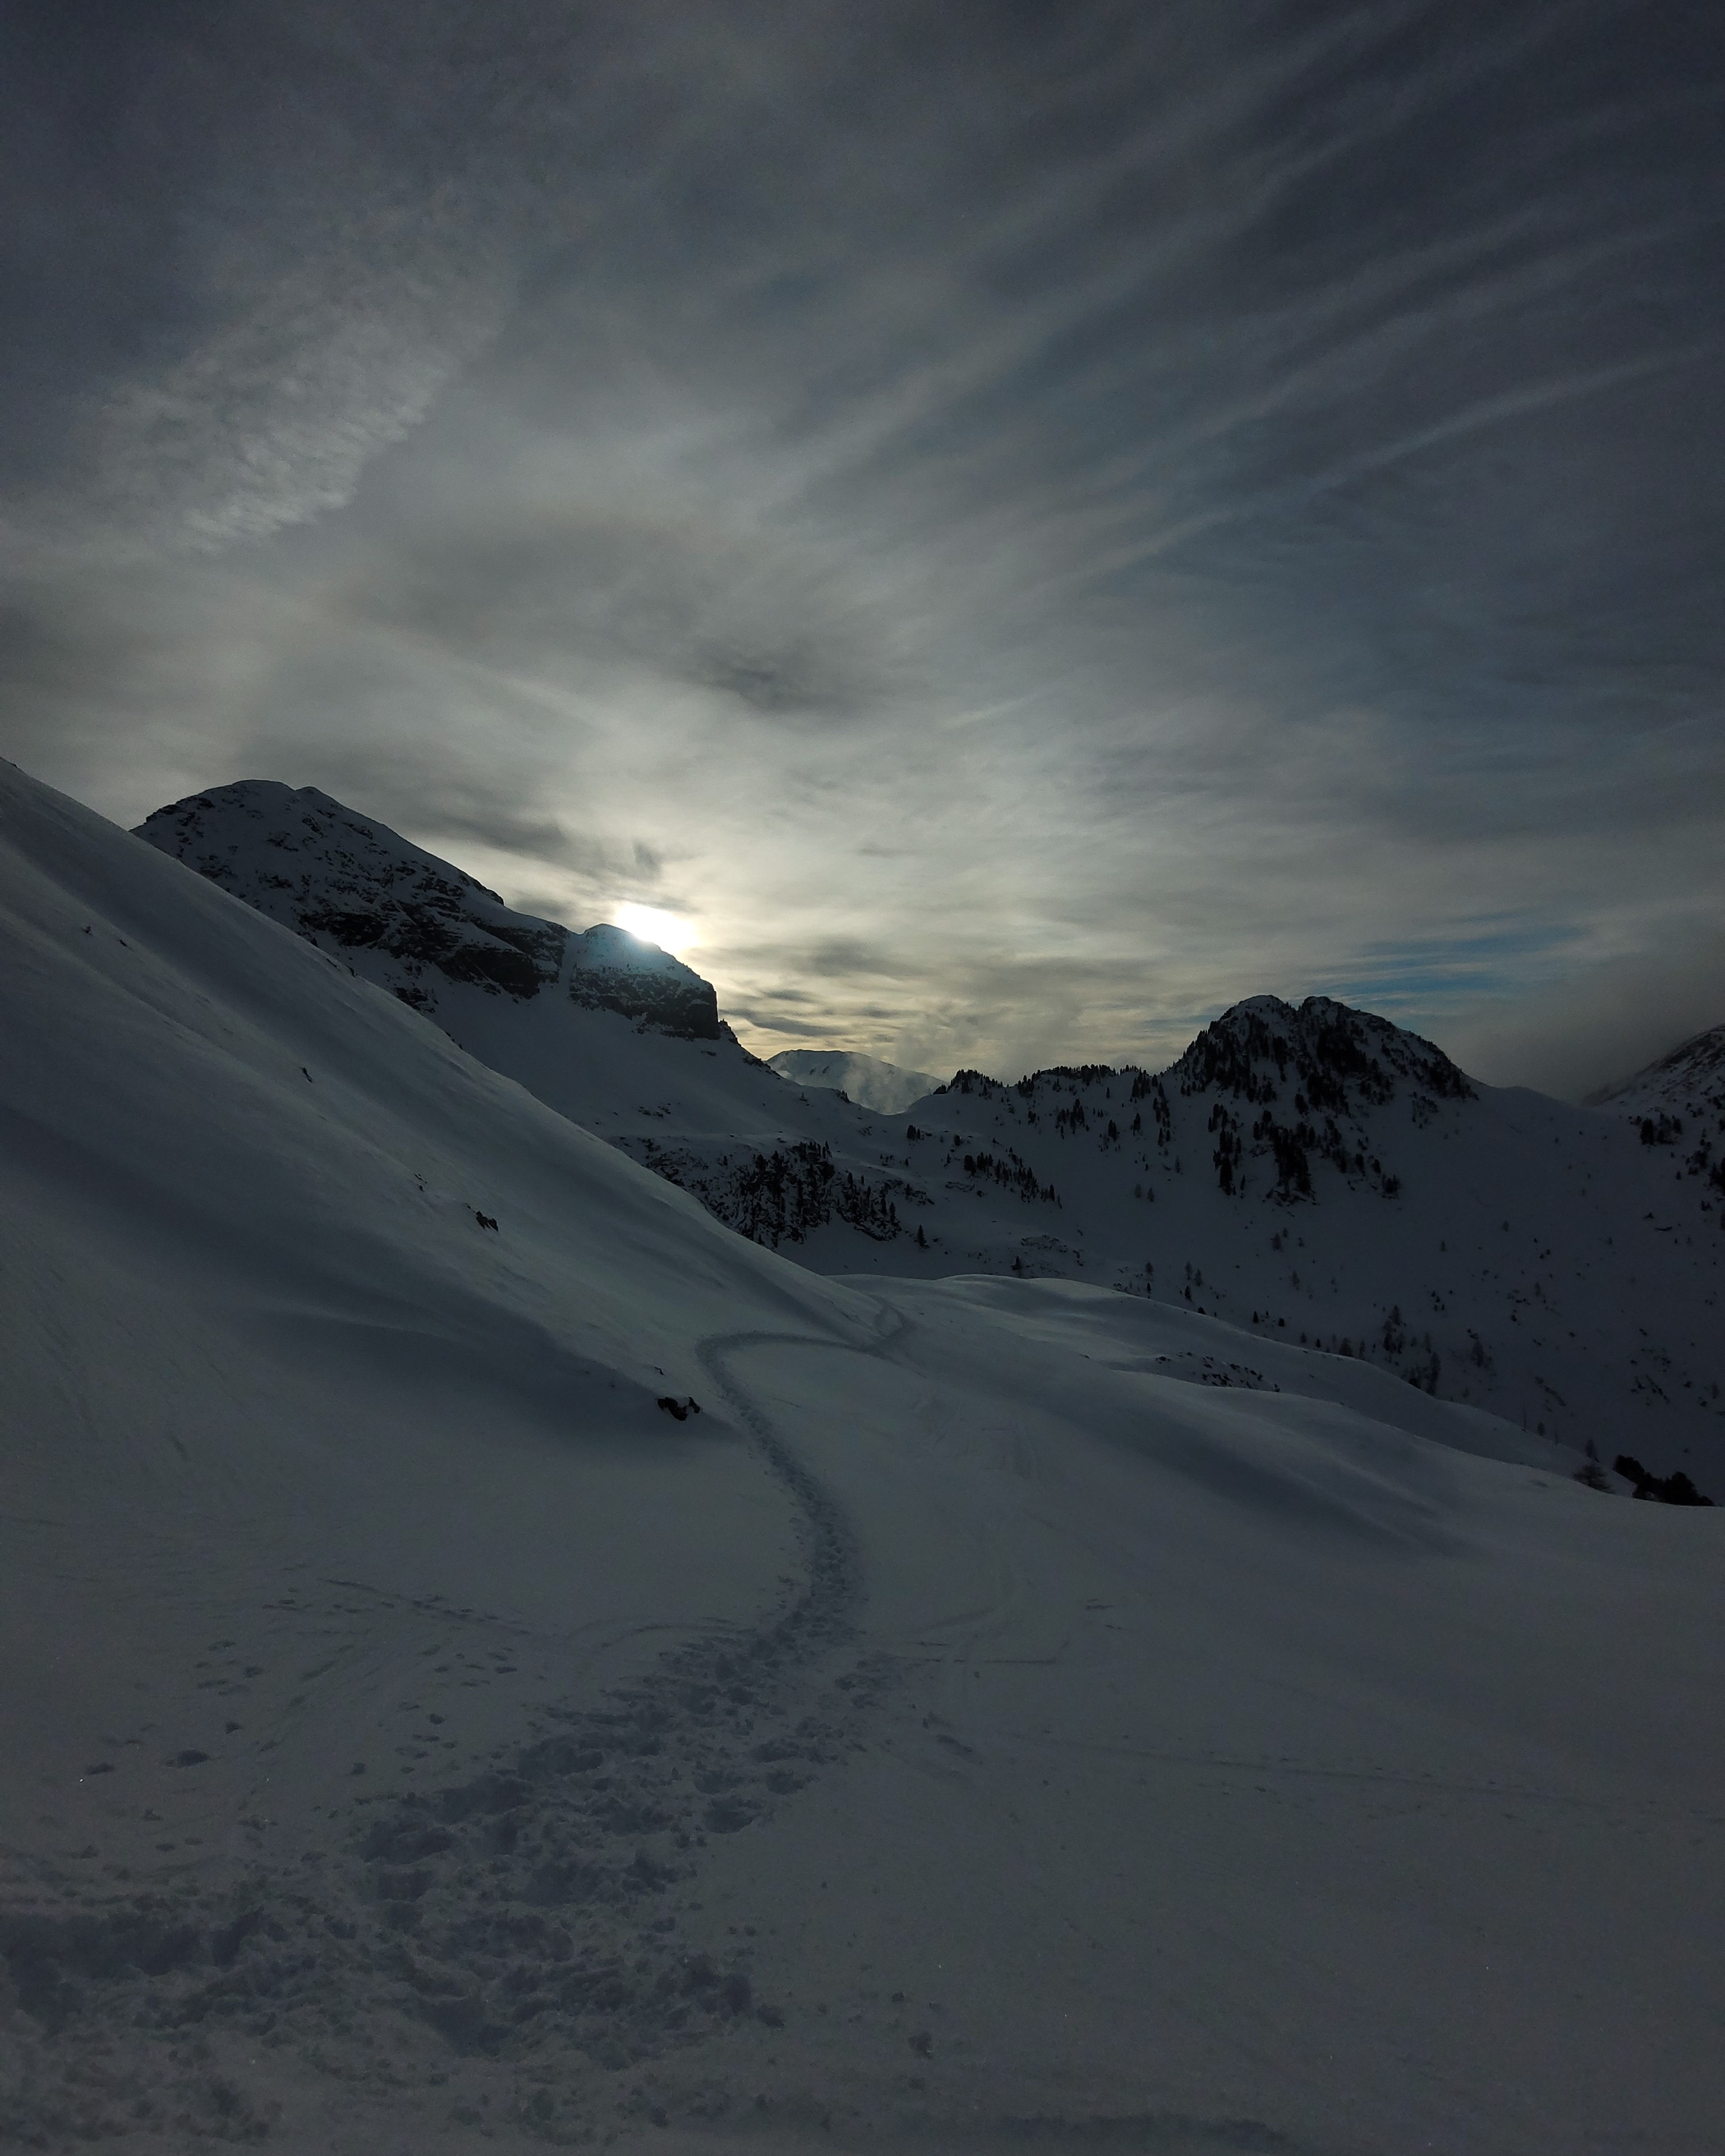
\includegraphics[width=\textwidth]{images/foto_sentiero.jpg}
        \caption{Sentiero sul monte.}
    \end{subfigure}
    \hfill
    \begin{subfigure}[b]{0.45\textwidth}
        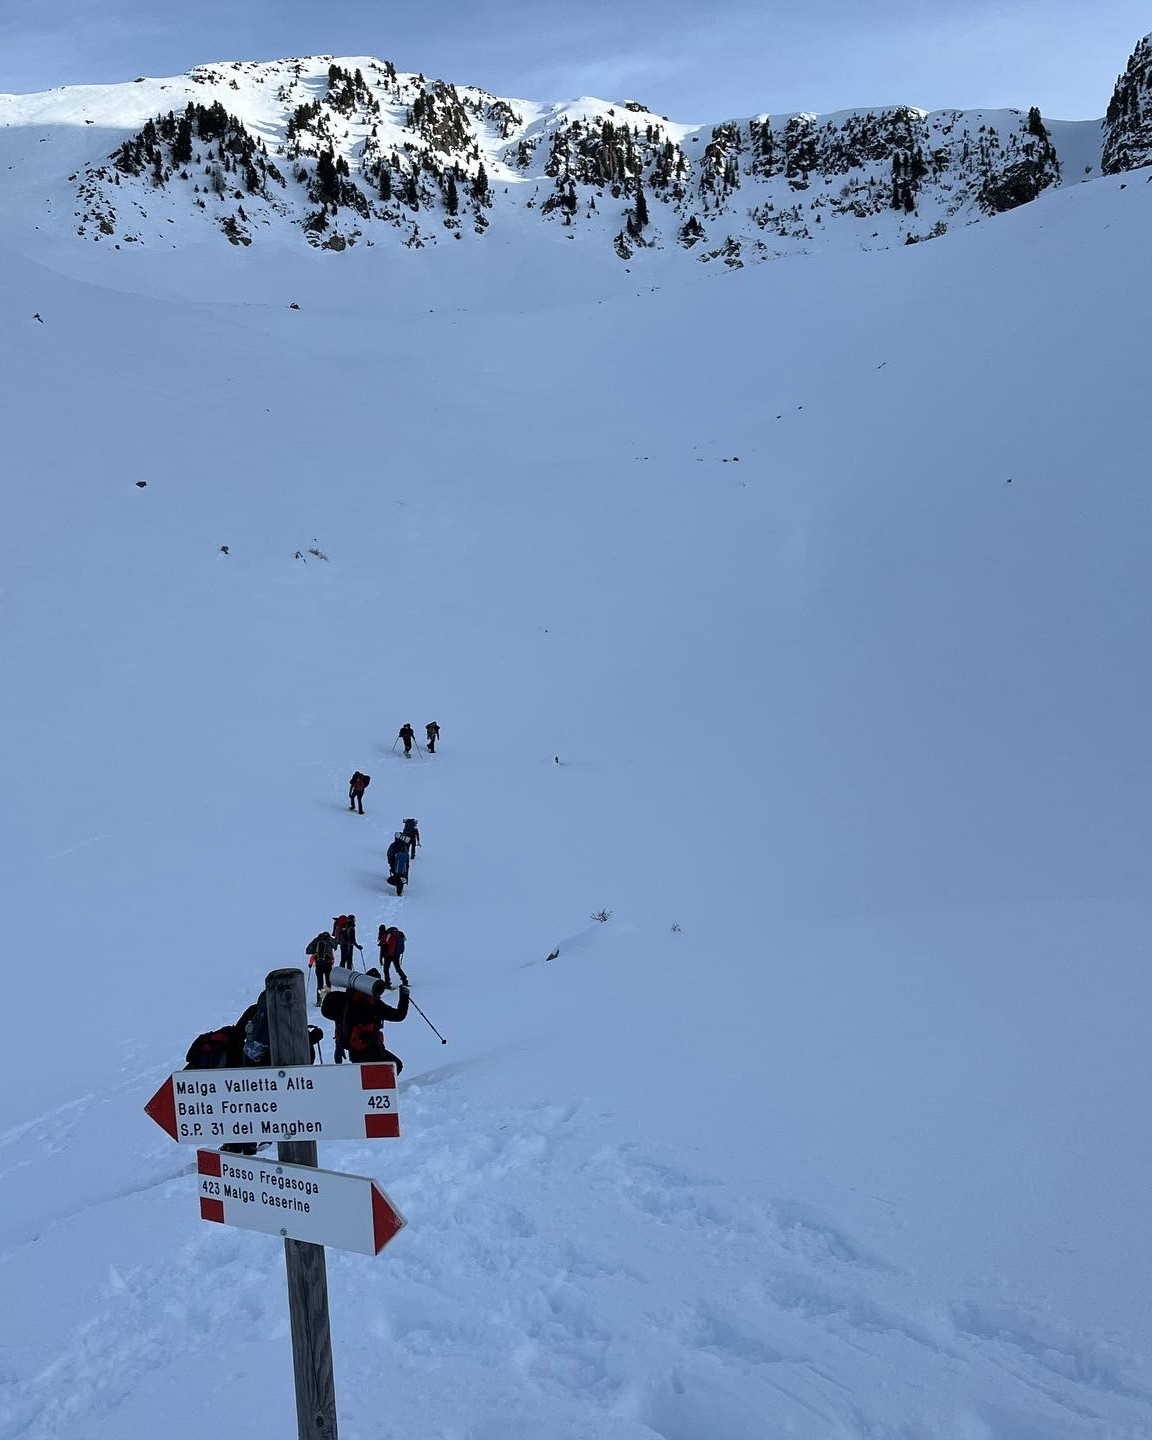
\includegraphics[width=\textwidth]{images/foto_sentiero2.jpg}
        \caption{Altro sentiero sul monte.}
    \end{subfigure}
    \hfill

    \caption{Selezione di fotografie del percorso e della vista dal bivacco.}
\end{figure}

\begin{figure}[H]
    \centering
    % Seconda riga: Tre foto (QUESTA È LA SECONDA FIGURA)
    \begin{subfigure}[b]{0.45\textwidth}
        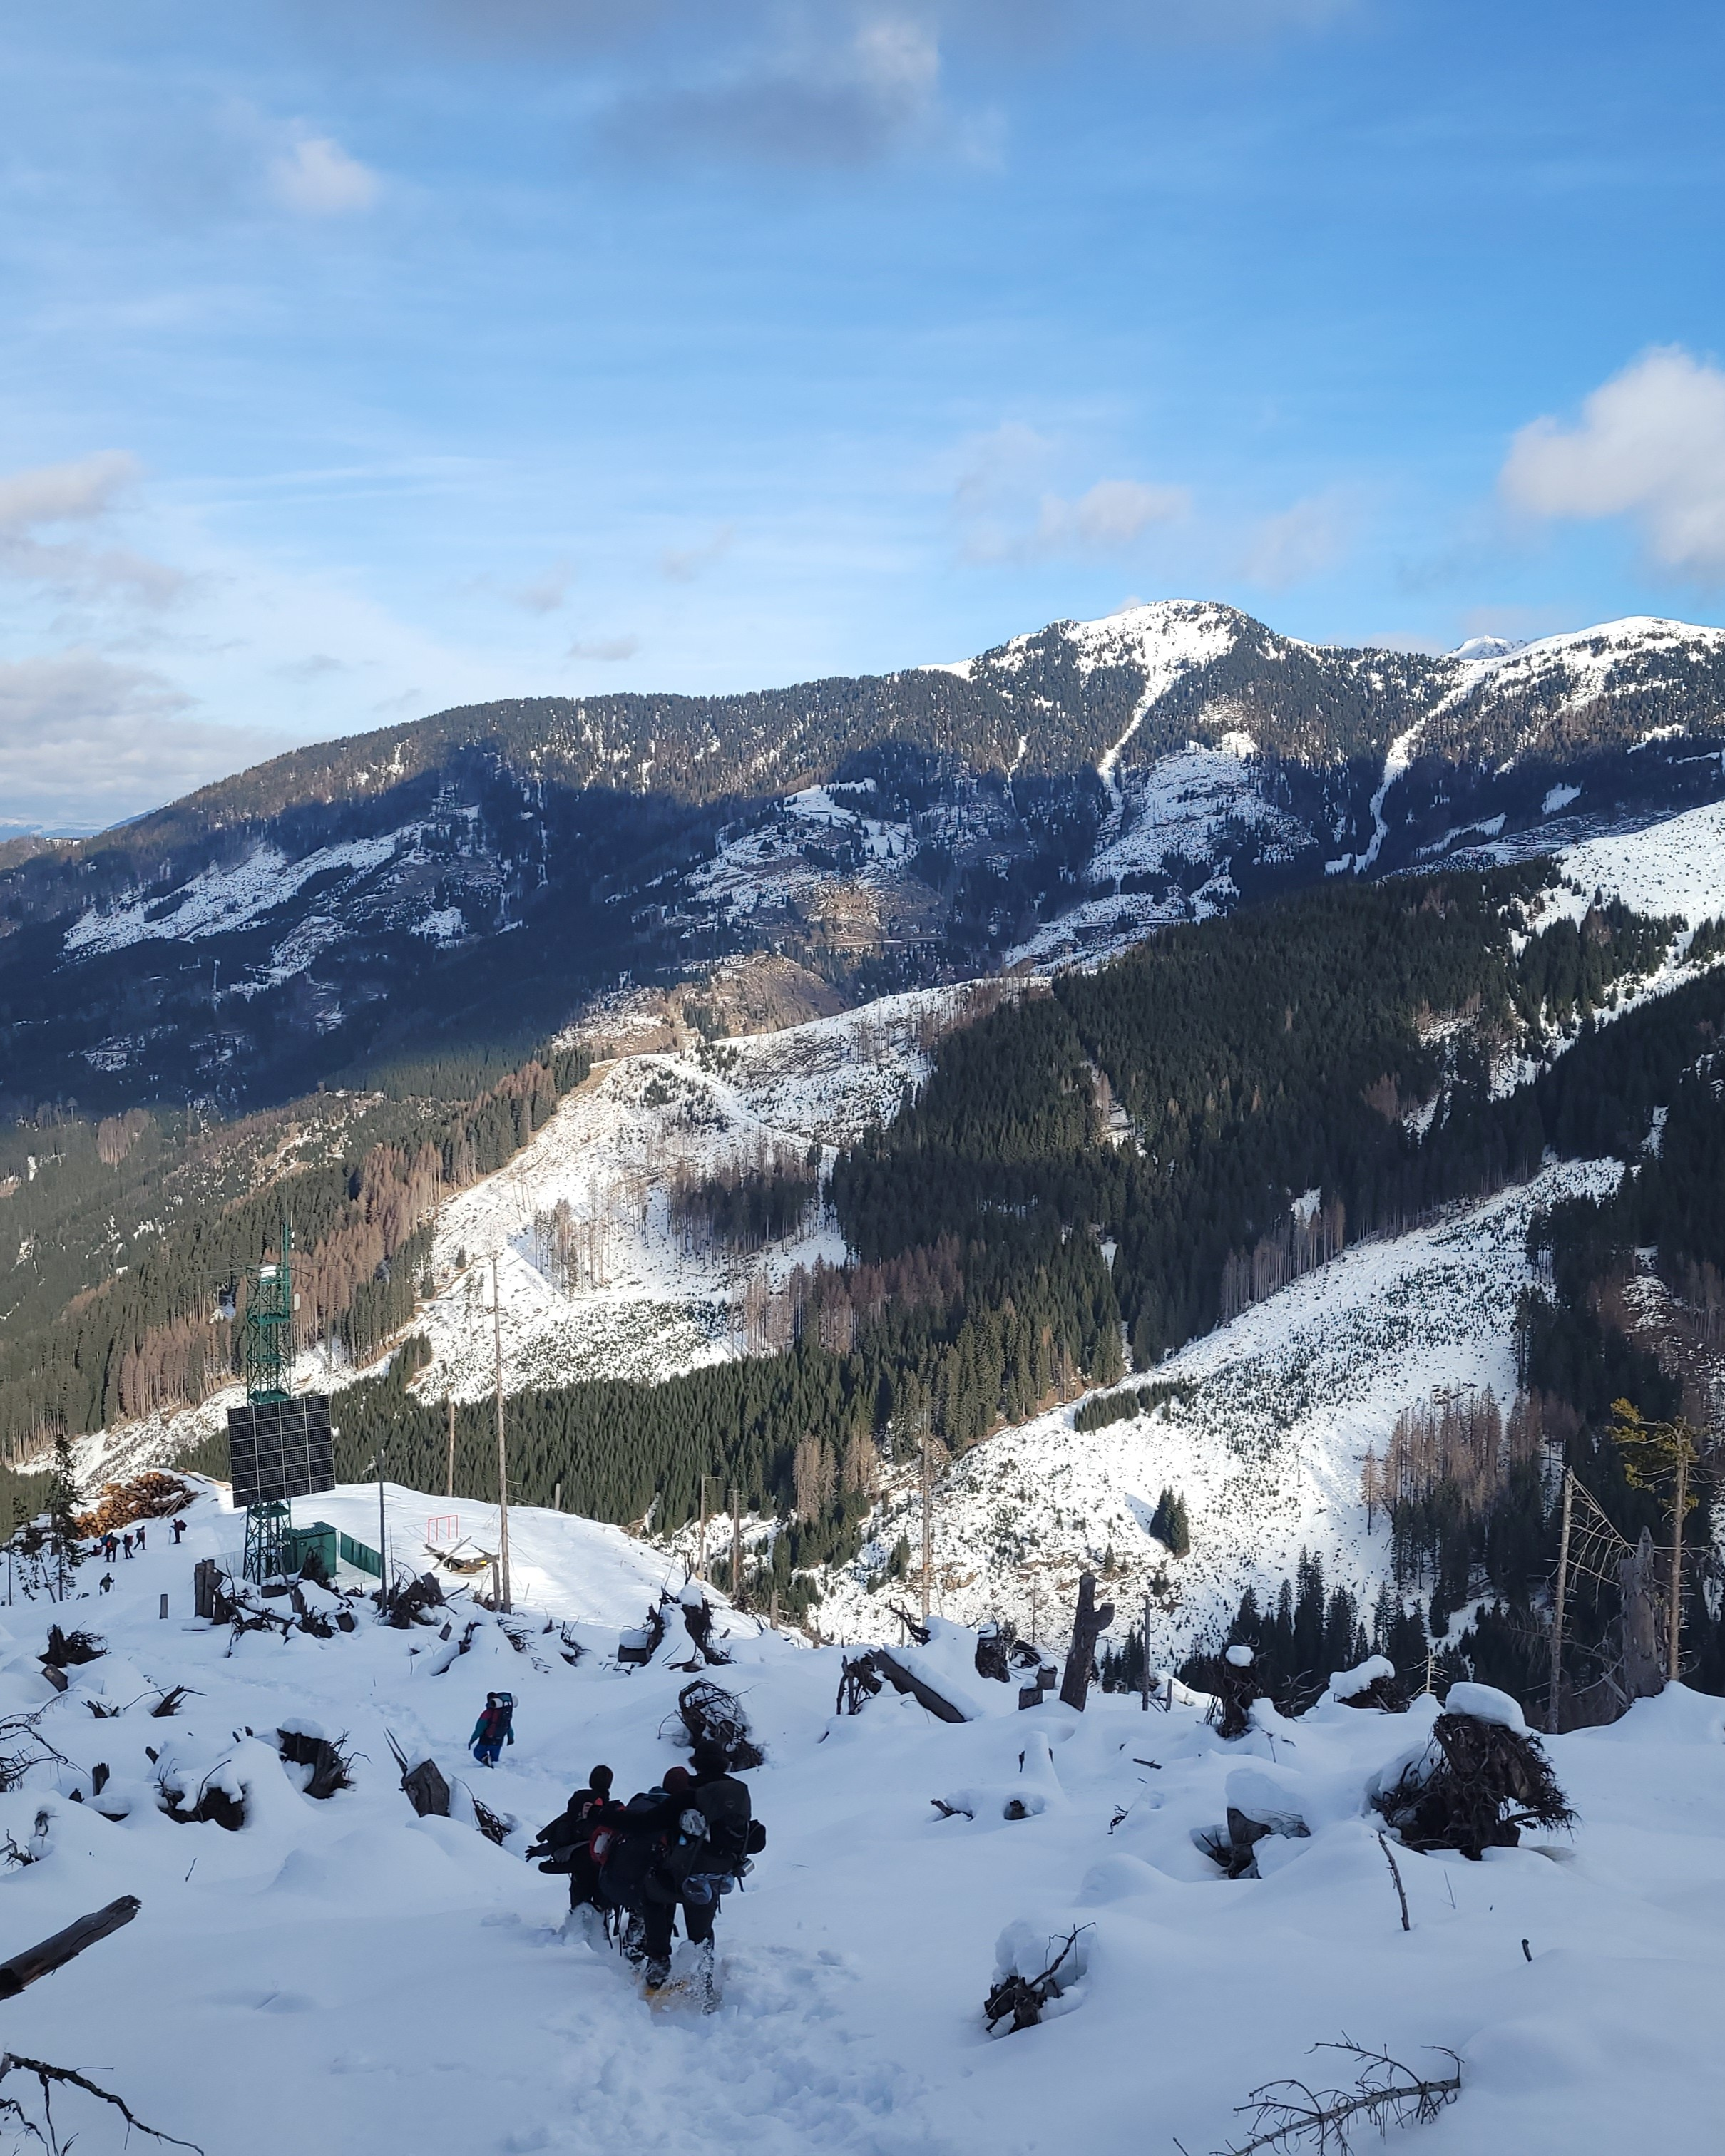
\includegraphics[width=\textwidth]{images/foto_paesaggio2.jpg}
        \caption{Altro paesaggio.}
    \end{subfigure}
    \hfill
    \begin{subfigure}[b]{0.45\textwidth}
        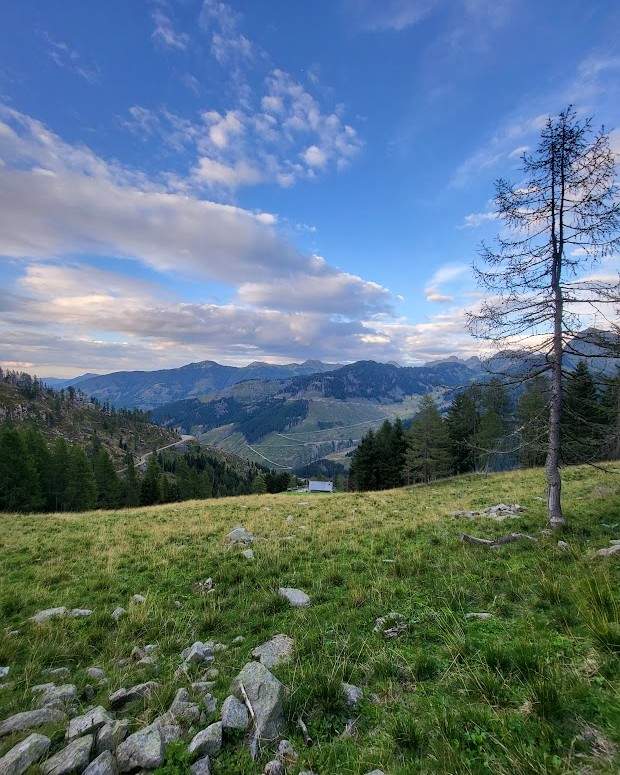
\includegraphics[width=\textwidth]{images/foto_estiva.jpg}
        \caption{Vista del bivacco.}
    \end{subfigure}
    \hfill

    \caption{Selezione di fotografie del percorso e della vista dal bivacco.}
\end{figure}

\begin{figure}[htbp!]
    \centering
    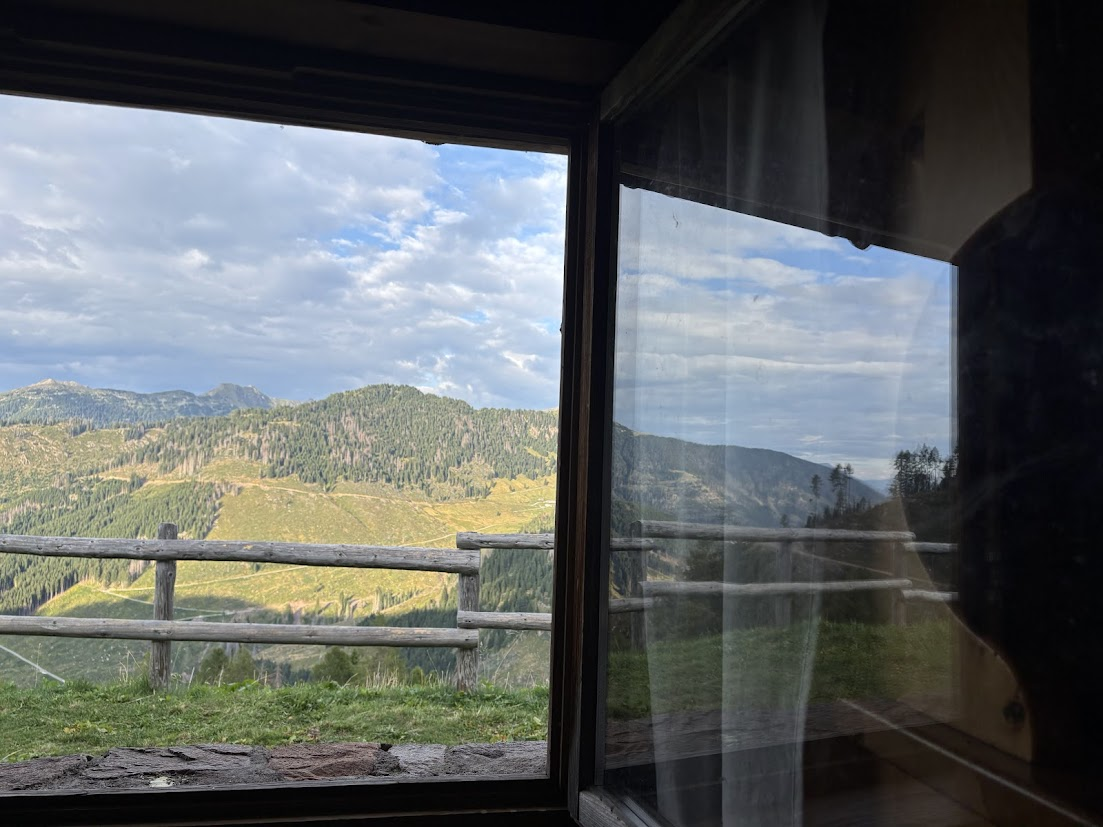
\includegraphics[width=\textwidth]{images/foto_finestra.jpg}
    \caption{Panorama visto dal bivacco.}
    \label{fig:foto_orizzontale}
\end{figure}


\end{document}
